%
% Chapter 4
%
\chapter{Solution Architecture}\label{chap:architecture}

The present chapter covers the system's components, their interactions, and the underlying technologies used to implement the solution. The architecture is designed to ensure data integrity, security, and scalability while providing a seamless user experience. We will cover the concept of a multiplatform application, how it functions, the various solutions available, and a detailed discussion of the chosen technology stack, specifically React Native with the Expo platform.

\section{Architecture Overview (CHAPTER UNDER DEVELOPMENT)}\label{sec:architecture-overview}

The architecture of the \texttt{DiGO Certify} system is designed to be modular, scalable, and secure. The system is divided into two main layers: the mobile application layer and the fully distributed layer. Each layer has specific responsibilities and interacts with the others to deliver the desired functionality.

\begin{figure}[H]
    \centering
    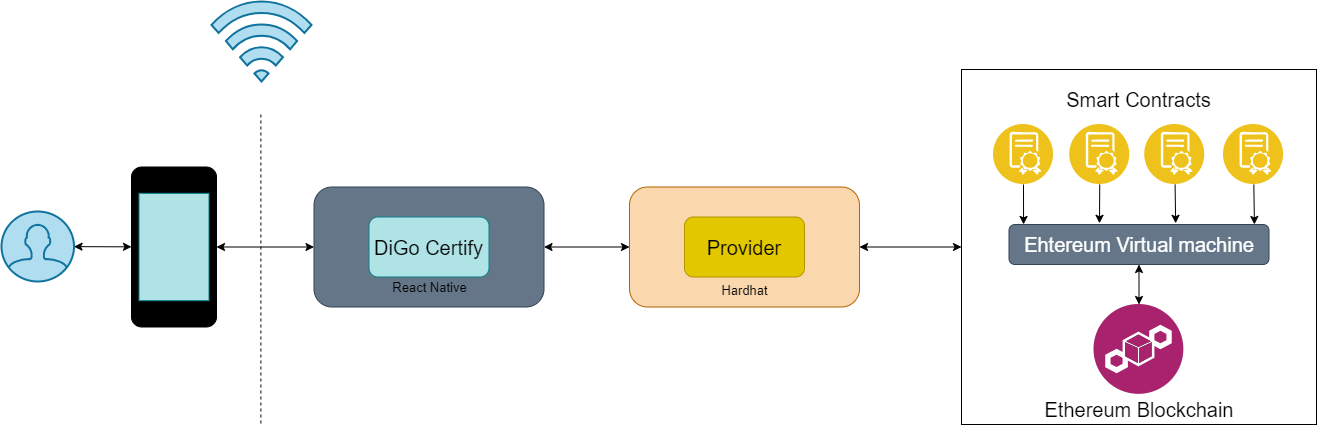
\includegraphics[width=1\textwidth]{assets/architecture-overview.drawio.png}
    \caption{Architecture Overview Diagram (inspired by \cite{geeksforgeeks-dApps}).}
    \label{fig:architecture-overview}
\end{figure}

...

\section{Fully Distributed Environment}\label{sec:fully-distributed-environment}

\section{Mobile Application}\label{sec:mobile-application}

\subsection{Multiplatform Application}\label{sec:multiplatform-application}

A multiplatform application is designed to run seamlessly on multiple operating systems, such as iOS and Android, using a single codebase. This approach significantly reduces development time and costs while ensuring a consistent user experience across different devices. The core idea is to write the code once and deploy it across multiple platforms, which is particularly beneficial for applications that need to reach a broad audience.

\subsubsection{Functionality and Operation}

Multiplatform applications leverage frameworks that provide tools and libraries to facilitate cross-platform development. These frameworks abstract away the differences between the various platforms, allowing developers to focus on building features rather than dealing with platform-specific nuances. The primary goal is to achieve native-like performance and look-and-feel while maintaining a shared codebase.

\subsubsection{Available Solutions}

Several frameworks are available for developing multiplatform applications, each with its own set of features and trade-offs. The most notable ones include:

\begin{itemize}
    \item React Native\cite{ReactNativeBook}
    \item Flutter\cite{Flutter}
    \item Kotlin Multiplatform Mobile (KMP)\cite{KMP}
\end{itemize}

\subsubsection{React Native}

React Native is a popular open-source framework developed by Facebook. It allows developers to build mobile applications using JavaScript and React, a widely-used library for building user interfaces. React Native bridges the gap between web and mobile development by enabling code reuse across platforms while providing near-native performance\cite{ReactNativeBook}.

\paragraph{Key Features:}

\begin{itemize}
    \item \textbf{Component-Based Architecture:} Enables modular and maintainable code.
    \item \textbf{Hot Reloading:} Allows developers to see changes in real-time without recompiling the entire application.
    \item \textbf{Rich Ecosystem:} A vast collection of libraries and tools that streamline development.
    \item \textbf{Community Support:} Extensive community contributions and support.
\end{itemize}

\subsubsection{Flutter}

Flutter, developed by Google, is another powerful framework for building natively compiled applications for mobile, web, and desktop from a single codebase. It uses the Dart programming language and provides a rich set of pre-designed widgets to create highly customizable interfaces\cite{Flutter}.

\paragraph{Key Features:}

\begin{itemize}
    \item \textbf{Hot Reload:} Similar to React Native's hot reloading, enabling quick iterations.
    \item \textbf{Expressive UIs:} Rich set of customizable widgets.
    \item \textbf{Performance:} Compiled directly to native code, which can lead to better performance.
\end{itemize}

\subsubsection{Kotlin Multiplatform Mobile (KMP)}

KMP, developed by JetBrains, allows developers to use Kotlin for developing iOS and Android applications. It focuses on sharing code, particularly business logic, while allowing platform-specific code where necessary\cite{KMP}.

\paragraph{Key Features:}

\begin{itemize}
    \item \textbf{Code Sharing:} Share common code across platforms while writing platform-specific code when needed.
    \item \textbf{Native Performance:} Utilizes native components and performance optimizations.
\end{itemize}

\subsection{Chosen Solution: React Native with Expo}

For the \texttt{DiGO Certify} application, we chose React Native with the \texttt{Expo} platform. This decision was influenced by several factors, including our team's familiarity with JavaScript and React, the maturity and stability of the React Native ecosystem, and the added benefits provided by Expo\cite{Expo}.

To make an informed decision, we compared several frameworks, including Flutter and Kotlin, based on various parameters:

\begin{table}[h]
    \centering
    \caption{Comparison of Flutter, React Native, and Kotlin.\cite{RNvsFluttervsKMP}}
    \begin{tabular}{|p{2.5cm}|p{4cm}|p{4cm}|p{4cm}|}
        \hline
        \textbf{Parameter}         & \textbf{Flutter}                           & \textbf{React Native}                             & \textbf{Kotlin}                                                        \\ \hline
        \textbf{Ease of Coding}    & Widget-based, reactive framework (Dart)    & JSX and JavaScript, component-based (React)       & Concise, expressive, reduces boilerplate (Kotlin)                      \\ \hline
        \textbf{Scalability}       & Good scalability, reactive architecture    & Scales well, may need native modules              & Excellent scalability, especially for large codebases                  \\ \hline
        \textbf{Performance}       & High performance, compiled language (Dart) & Near-native performance, native modules if needed & Efficient performance, native language for Android                     \\ \hline
        \textbf{Learning Curve}    & Moderate, widget-based approach            & Relatively easy for JavaScript developers         & Moderate, especially for those familiar with Java                      \\ \hline
        \textbf{Popularity}        & Growing rapidly, gaining popularity        & Widely adopted, mature, and well-established      & Highly popular for Android development                                 \\ \hline
        \textbf{Stability}         & Stable, regular updates and improvements   & Stable, backed by Facebook and active community   & Stable, regular updates and improvements                               \\ \hline
        \textbf{Types of App Dev}  & Cross-platform focus for consistent UI     & Cross-platform, leverages JavaScript expertise    & Primarily for native Android; Kotlin Multi Platform for cross-platform \\ \hline
        \textbf{Community Support} & Growing community support                  & Large and active community support                & Strong support, especially in the Android community                    \\ \hline
    \end{tabular}
\end{table}


React Native’s component-based architecture aligns well with our need for a modular and maintainable codebase. Our team’s existing knowledge of JavaScript and React significantly reduced the learning curve, allowing us to quickly become productive and focus on delivering features. Compared to Flutter and Kotlin, React Native's learning curve is relatively easy for JavaScript developers, while Flutter requires learning Dart, and Kotlin, despite being expressive and reducing boilerplate, may be more moderate for developers familiar with Java.

In terms of performance, React Native provides near-native performance, ensuring that our application runs smoothly on both iOS and Android. This is similar to Flutter, which offers high performance through its compiled language, Dart, and Kotlin, which provides efficient performance for native Android development. However, React Native can scale well with the potential need for native modules, providing flexibility in development.

The framework’s rich ecosystem of libraries and tools further accelerated our development process, providing pre-built components and solutions that we could easily integrate into our application. The extensive community support for React Native ensured that we had access to numerous resources, tutorials, and third-party libraries, which proved invaluable during the development process. This support network allowed us to quickly troubleshoot issues and implement best practices, contributing to a more efficient development cycle. While Flutter's community is rapidly growing, React Native's community is already large, mature, and well-established, and Kotlin also enjoys strong support, especially in the Android community.

Expo enhances React Native by offering a suite of tools and services that simplify development. With Expo, we benefit from an integrated environment for developing, building, and deploying React Native applications. The platform’s managed workflow handles many of the complexities of building and deploying mobile applications, allowing us to focus on developing features rather than dealing with infrastructure. Expo’s easy setup and configuration process streamlined our project initialization, while its over-the-air update capability enables us to push updates to users without requiring a full app store review process.

The development workflow for DiGo Certify using React Native and Expo involves several key steps. Initially, we set up the project with Expo CLI, which provides a streamlined setup process and essential tools. We then focused on building the application UI using React Native’s component-based approach. This method allows us to create reusable UI elements that help maintain consistency and simplify development.

For integrating blockchain functionality, we implemented smart contracts in Solidity and connected them with the React Native application through ethers.js. This integration enables secure interactions with the Ethereum blockchain, allowing for the storage and validation of academic certificates.

Testing and debugging are facilitated by Expo’s built-in tools, which allow us to test the application on various devices and simulators. This ensures that our application performs well across different platforms and devices. Finally, Expo simplifies the deployment process with its build and publish services, allowing us to distribute the application through app stores seamlessly.

In summary, the choice of React Native with Expo for DiGo Certify provides a robust, efficient, and scalable solution for developing a secure and user-friendly multiplatform application. This architecture leverages modern technologies to meet the needs of our diverse user base, ensuring a high-quality user experience across all supported devices.